\documentclass[9pt,serif]{beamer}
\usepackage[]{tikz}
\usepackage[]{graphicx}
\usepackage[]{float} 
\usepackage[]{import}
\usetheme{Rochester}
\usepackage{graphicx}
\usepackage[]{amsthm,amssymb,amsmath}


%

\usepackage[icmcb]{mycolors} 
\usepackage{verbatim}


    \usepackage{thmtools, listings, chngcntr}
    \usepackage[most]{tcolorbox}
    \usepackage{ifthen, xifthen}
    \usepackage[framemethod=TikZ]{mdframed}

%This code is made for Itemized portions
\newenvironment{myitemize}{\begin{itemize}}{\end{itemize}}
    \tcolorboxenvironment{myitemize}{blanker, before skip=6pt,after skip=6pt,
borderline west={2mm}{0pt}{red}} 

    \declaretheoremstyle[ headfont=\bfseries\color{black}, notebraces={[}{]},
    notefont=\normalfont\sffamily, headpunct={. }, spaceabove=10pt,
    spacebelow=10pt, qed=\qedsymbol, bodyfont=\color{black}, ]{solutionstyle}

\tcolorboxenvironment{solution.}{ coltext=solC!90!pageC, tile, breakable,
colback=pageC, top=0pt, left=.7em, right=.7em, before skip=0pt,after
skip=35pt,borderline west={.1em}{0pt}{solC}, }
\declaretheorem[style=solutionstyle]{solution.} \newtheorem*{solution.*}{Sl}


        \declaretheoremstyle[ headfont=\bfseries\color{Olive Green},
        headpunct={.}, postheadspace={7pt}, spaceabove=12pt,
        bodyfont=\normalfont, spacebelow=12pt, notebraces={(}{)},
        notefont=\color{probC}, ]{ideastyle}


\tcolorboxenvironment{idea}{ tile, breakable,colback=defBgC, colframe=probBgC,
coltext=fgC, left=1em,before skip=12pt,after skip=30pt, borderline
west={2mm}{0pt}{gray}, } \declaretheorem[style=ideastyle]{idea}
\newtheorem*{idea*}{id}


        \declaretheoremstyle[ headfont=\bfseries\color{probC}, headpunct={.},
        postheadspace={7pt}, spaceabove=12pt, bodyfont=\normalfont,
        spacebelow=10pt, notebraces={(}{)}, notefont=\color{probC},
        ]{problemstyle}


\tcolorboxenvironment{problem.}{ tile, breakable,colback=probBgC,
colframe=probBgC, coltext=fgC, left=1em,before skip=12pt,after skip=30pt, }
\declaretheorem[style=problemstyle]{problem.} \newtheorem*{problem.*}{Pr}

         \newcommand{\solu}[1]{ \begin{solution.} #1 \end{solution.} }
         \newcommand{\prob}[1]{ \begin{problem.} #1 \end{problem.}}

        \newcommand{\id}[1]{ \begin{idea} #1 \end{idea} }
%_{_{_{_{_}}}} Macros are here 
\newcommand{\fig}[3]{ \begin{figure} \centering \includegraphics[width=
#1\textwidth]{#2} \caption{#3}  \end{figure}} 
%
\newcommand{\draw}[3]{ \begin{figure}[hbt!] \centering
 \fontsize{35pt}{20pt}\selectfont \resizebox{#1 \textwidth}{!}{
\import{}{#2.pdf_tex}}\caption{#3} \label{#3} \end{figure} }
%_{_{_{_{}}}}}

\newcommand{\sides}[2]{ \begin{minipage}{0.5\textwidth} #1
    \end{minipage}\hfill%
\begin{minipage}{0.5\textwidth} #2 \end{minipage} }
\usepackage[]{xcolor}
 \usepackage[]{pdfpages}
 \usepackage[]{transparent}
 \usepackage[]{xifthen}
\newcommand{\incfig}[1]{ 
\fontsize{ 35pt}{ 20pt}\selectfont \resizebox{0.6\textwidth}{!}{ 
\import{./figures/}{#1.pdf_tex} } 
} 

\title{Day 1} \author{Ahmed Saad Sabit} \date{\today} 



\begin{document}

% this is the title page.
\begin{frame}{Intro} \titlepage  \end{frame}

% quick intro to sin and cos 
\begin{frame}{0.1 Right Angled Triangle - The Triangle with a $90^{\circ}$. }
\fig{0.6}{f1.png}{Right Angled Triangle}  \end{frame}

\begin{frame}{0.2 Trig} Because of some ratio of the right angled triangle we
    can say that, \[ \sin \theta = \frac{\text{Opposite}}{\text{Hypotenuse}} \]
    \[ \cos \theta = \frac{\text{Adjacent}}{\text{Hypotenuse}} \]
  
    
\end{frame}

\begin{frame}{0.3 Measuring Angles} \draw{0.5}{drawing2}{Comaparison} This
    means that, \[ 180^{\circ} = \pi \ \text{radians} \] The reason we use
radian can be shown when needed.  \end{frame}



\begin{frame}{0.4 The fact $\alpha + \beta + \gamma = 180^{\circ} =  \pi$ } If
    you add all angles inside a triangle, the sum will always be $180^{\circ}$.
    \draw{0.4}{180angle}{Summing up angles} \[ \alpha + \beta + \gamma =
    180^{\circ} =  \pi \] For a right angle triangle, $\gamma = 90^{\circ} =
    \frac{\pi}{2}$, hence, \[ \alpha + \beta + 90^{\circ} =  180 ^{\circ} \]\[
\alpha + \beta =  90^{\circ}\]
       

\end{frame}


% we are going to solve problems from this part
% 
% 
% 









\begin{frame}{Newton`s Second Law: $\vec F =  m \vec a$ }

    \draw{0.6}{N2L-1}{If you push a block}
    
\end{frame}





\begin{frame}{N2L}

    \draw{0.6}{N2L-2}{The movement will be in the same direction}

    The movement is Acceleration. Acceleration is increase/decrease in speed
    overtime.  \[ \vec{a} = \frac{\mathrm d \vec v}{\mathrm d t} \]
    
\end{frame}



\begin{frame}{A required relation of angles $\alpha$ and $\beta$.}
    \draw{0.8}{prob1-8}{}    

\end{frame}



\begin{frame} \begin{minipage}{0.5\textwidth} \draw{1}{prob1-9}{}
\end{minipage}%
\hfill \begin{minipage}{0.5 \textwidth} This actually shows us
that, \[ r \sin \alpha =  r \cos \beta \] \[ r \cos\alpha = r \sin\beta \]
\pause Because $\alpha + \beta = 90^{\circ}$, $\beta =  90^{\circ} -\alpha$.
Hence, \[ r \sin \alpha =  r \cos ( 90^{\circ} - \alpha) \] \[ r \cos\alpha =
r \sin (90^{\circ} - \alpha)  \] \pause So, we now know that, \begin{align*}
\sin(90^{\circ} - \alpha ) = \cos \alpha \\ \cos(90^{\circ} - \alpha) =
\sin\alpha \end{align*} \end{minipage} \end{frame}
%
%
%
%
%
%
\begin{frame}
    {Warm Up: Cosine Law --- For Vector}
    \sides{
   We will use vectors very often in physics, so it is better we try it out before starting.
    At first, vectors can be added in this way, \\
    Vectors can be added, like, 
    \[ \vec a + \vec b \]
Which looks like one vector is put infront of another. }{
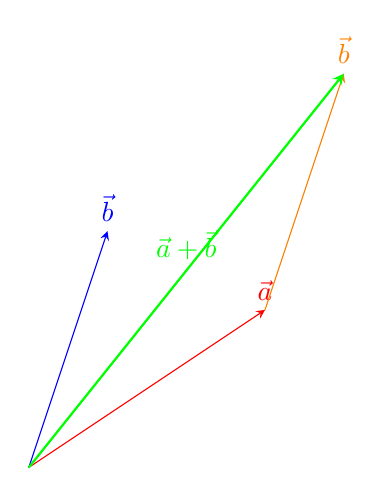
\begin{tikzpicture}
    \centering
    \draw[-stealth, red](0,0) -- (3,2) node[above]{$\vec{a}$};\pause
        \draw[-stealth, blue](0,0) -- (1,3) node[above]{$\vec{b}$};\pause
            \draw[-stealth, orange](3,2) -- (4,5) node[above]{$\vec{b}$};\pause
                \draw[-stealth, thick, green](0,0) -- (4,5) node[midway, above]{$\vec a + \vec b $ };
\end{tikzpicture}
}
\end{frame}
%
%
%
%
%
%

\begin{frame}
    {Vector Triangle for Cosine Law}
    \sides{If there is a side $a$ and $b$, then assuming the third side is $c$, the Law of cosine is to find the length of $c$ using the lengths of $a$ and $b$, and the angle $a$ and $b$ makes. \\
    The easiest solution can be found using $\vec a$ and $\vec b$ vector methods. We know angle $\theta$ between $a$ and $b$ }{
    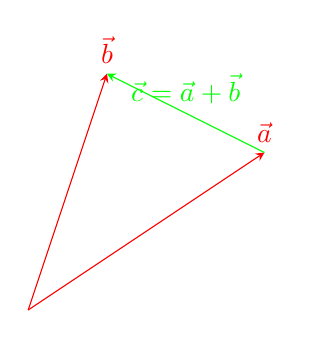
\begin{tikzpicture}
        \centering
        \draw[-stealth, red](0,0) -- (3,2) node[above]{$ \vec a$}; 
        \draw[-stealth, red](0,0) -- (1, 3) node[above]{$\vec b $};
        \draw[-stealth, green](3,2) -- (1,3) node[midway,above]{$\vec c= \vec a + \vec b$};
\end{tikzpicture}}
\end{frame}


\begin{frame}
    Now let us have a triangle with side $\vec a$ and $\vec b$, then the third side is obviously $\vec b - \vec a$. This is same as we saw in last frame. Now, let the third side be $\vec c = \vec b - \vec a$, then can we find a scalar solution for the length of vector $\vec c$?\\
    \begin{align*}
        \vec c &= \vec b - \vec a \\    \pause
        \left(  \vec c \right) ^2 &=  \left( \vec b - \vec a \right) ^2 \\ \pause
        \vec c \cdot \vec c &= \vec a \cdot \vec a -
        2 \vec a \cdot \vec b +
        \vec b \cdot \vec b 
    \end{align*}
    Now, $\vec a \cdot \vec b$, is the dot product. And for a dot product, 
    \[ \vec a \cdot \vec b = |a| \ |b| \ \cos \theta  \] \pause
    And if, 
    \[ \vec a \cdot \vec a = |a| |a | \cos \left( 0 \right)  \] \pause
    Because $\vec a$ makes $0 ^{\circ}$ with itself. Hence, we have, 
    \[ c^2 = a^2 + b^2 - 2ab \cos\theta \]
    So, we have found length of third side,  \[ c=
    \sqrt{a^2 + b^2 - 2ab \cos \theta}  \]
     
\end{frame}


\begin{frame}{Sine Law}
\sides{\begin{small}
\textbf{\textsf{The $\sin \alpha$ Law:}} For a triangle, with lowercase denoting the angle and the uppercase the opposite side, the sides and angle follow the relation respect to the circumcircle is that, 
\[ \frac{a}{\sin A} \,=\, \frac{c}{\sin C} \,=\, \frac{d}{\sin D} \, = \, 2r\]
\textbf{\textsf{Proof:}} Let $\triangle ACD$ be the required triangle, we want to build a relation between the length of the sides and the opposite angles to them motivated from the fact that the opposite angle being large making the side project a larger length.
\end{small}}{
\fig{0.8}{sinelawpic.png}{Sine Law}

}

\end{frame}


\begin{frame}
\fig{0.8}{sinelawpic.png}{Sine Law}
\end{frame}



\begin{frame}
 Let $\Gamma$ be the circumcircle of $\triangle ACD$ and we draw a diameter $DE$ that passes through the center of $\Gamma$ which is point $O$. \\
 $\triangle ECD$ is a Right Angled Triangle because it meets the \emph{Semi-circle} and thus,
 \[ \sin \angle CED = \frac{\Bar{CD}}{\Bar{ED}}\]
 Using the \emph{Arc and Angle Theorem} we can see that  
 \[ \angle CED = \angle CAD = \angle A \]
 As we know that $DE = 2r$ we are left to show that,
 \begin{align}
 \sin \angle CED &=  \frac{\Bar{CD}}{\Bar{ED}} \notag \\
 \sin \angle A & = \frac{a}{2r} \\
 \frac{a}{\sin A} & = 2r
 \end{align}
 And this can be again and again be proved for all the three remaining sides,
 \begin{equation}
 \frac{a}{\sin A} \,=\, \frac{c}{\sin C} \,=\, \frac{d}{\sin D} \, = \, 2r
 \end{equation}
 And we are done with the proof.
\end{frame}



\begin{frame}{Problem 1: The General Problem of Force}

    \prob{There is a system made of an incline with two masses attached with
    string as shown. One is $m_1 $ another is $ m_2$, gravity works $\vec{g}$.
\emph{Find the acceleration of both bodies  $m_1$ and $m_2$. }}  
    
    \draw{0.6}{prob1-1}{Problem 1 Diagram} 

\end{frame}




\begin{frame}{Problem 1: The General Problem of Force}

    \prob{There is a system made of an incline with two masses attached with
    string as shown. One is $m_1 $ another is $ m_2$, gravity works $\vec{g}$.
\emph{Find the acceleration of both bodies  $m_1$ and $m_2$. }}
\begin{minipage}{0.4\textwidth}
       
    \draw{0.8}{prob1-1}{Problem 1 Diagram} 

   \end{minipage} \hfill 
   \begin{minipage}{0.5 \textwidth}
   \begin{small}
       he main force is caused by Gravity \pause
The rope can pull the $m_2$ and slow down $m_1 $ when it tries to fall down. \pause
  here is possibility that too much pull be $m_2$ can cause the $m_1 $ to lift off the ground, instead of falling down. 
  We have to be careful about all the possibilities.
     \end{small} 
   \end{minipage} 
   \end{frame}







\begin{frame} This is the approach
    \begin{myitemize} 
    \item Find all the forces,
it's the tricky part. \pause 
    \item Find the acceleration from the force using
$\vec F =  m \vec a$.  i
\end{myitemize}

\end{frame}




\begin{frame}{Problem 1: Find All the forces}

    \draw{0.6}{prob1-2}{Sorry for this exploded word size.} We will start
isolating the force on the bodies $m_1 $ and $m_2$.  \end{frame}



\begin{frame}{Problem 1: Let us find the forces on $m_2$ first}
\draw{0.8}{prob1-3}{} \end{frame}




\begin{frame}{Problem 1: Let us find the forces on $m_1$ then}
\draw{0.8}{prob1-4}{} \end{frame}

\begin{frame}{What is $T$?} \begin{myitemize} \item    $T$ is the Tension
force, the ``Tan" (in Bengali) because of the rope.  \item $T$ is same for the
whole rope, otherwise a non zero force on the rope would occur.
\end{myitemize} \end{frame}



\begin{frame}{Let us look the total force on $m_2$ } Note that motion of the
    body $m_2$ is constrained (limited) in the incline.\draw{0.6}{prob1-5}{}
    Thus, there force on $ m_2$ can only work along the incline. This is force
    is made from $2$ components.  \end{frame}




\begin{frame} \draw{0.7}{prob1-6}{} \end{frame}

\begin{frame}
    \draw{0.5}{prob1-7}{} 
    \[ \alpha + \beta = 90^{\circ} \] And you
can note that the projection of the  $m_2 g$ vector has similar angles.
\end{frame}

\begin{frame}{On $m_2$ }

    \begin{minipage}{0.5\textwidth} 
        \begin{myitemize}   
        \item        We don't
        need the perpendicular force components. 
    \item       Because the block
        $m_2$ is constrained to move along the incline. 
    \item            So
        the force perpendicular to the motion are useless.  \end{myitemize}
    \end{minipage}\hfill
    \begin{minipage}{0.5\textwidth} \draw{1}{prob1-7}{}
\end{minipage}
    
\end{frame}

\begin{frame}{Sign Conventions for Problem} \sides{ We will consider the sign
        convention so that, \begin{myitemize} \item If $m_1$ falls down, then
            the motion is in positive direction.  \item If $m_1$ lifts up, the
            the motion is in negative direction.  \item $m_1$ falling down
        means that $m_2 $ will lift up along the ramp. This motion, where $m_2$
    will lift up along the inline/ramp, means the motion is ``Positive".
\end{myitemize} }{ \draw{1}{prob1-7}{} }



\end{frame} \begin{frame} \sides{ The force by gravity, parallel to the
direction of possible motion, \[ m_2 g \cos\beta = m_2 g \sin\alpha =  F_g \]
This is what we need. }{ \draw{1}{prob1-7}{}} \end{frame}


\begin{frame} \sides{ Now, the total force on $m_2$, \[ T - F_g  \] This total
    force can let us know about the accelearation of the $m_2$ using $F = ma$,
    \[ m_2 a_2 = T - F_g \]
        
    }{\draw{1}{prob1-7}{}} \end{frame}



\begin{frame} Now, we need the total force on $m_1$.  \end{frame}



\begin{frame} \sides{ The gravity pulls by $m_1 g$ and the tension pulls
    against $T$, so total force, \[ m_1 a_1 =  m_1 g - T \] }{
    \draw{1}{prob1-4}{} } \end{frame}

    

\begin{frame} 
    \sides{ 
        We have built up two equations, 

        \begin{align*} m_1 a_1 &=
        m_1 g - T \\ m_2 a_2 &=  T - m_2 g \sin\alpha    
    \end{align*}
        \begin{myitemize} 
        \item There are 2 equations 
        \item But there are 3
            unknowns. They are, $a_1, a_2, T$.  
        \end{myitemize} 
        This system of
        equation can only be solved if, The number of Unknown
        {\color{cyan}variable} match with the number of {\color{red}equations}. \\
    This means, \\ We need \emph{another} equation}
    {\draw{1}{prob1-7}{}}
    \end{frame}
%
%
%
%

%
%
\begin{frame}
\sides{
    Please look at $a_1$ and $a_2$, note that, because of the string, \\
both of the blocks $m_1$ and $m_2$ should together, in the same motion. \\
Because, if one is faster than the other, the rope will resist that. \\
So we shall have $a_1 = a_2$.
}
{
\draw{1}{prob1-7}{ }   
} { } 
\end{frame}
%
%
%
%
%
\begin{frame}{ Answer final} 
    Now using the fact $a_1 = a_2 = a$, 
        \begin{align*} m_1 a &=
        m_1 g - T \\ m_2 a &=  T - m_2 g \sin\alpha    
    \end{align*}
    To solve this equations, 
    \begin{itemize}
        \item $T = m_2 a + m_2 g \sin\alpha $ \pause
        \item Put this in second equation, $  m_1 a = m_1g - \left( m_2 a + m_2 g \sin\alpha  \right)      $. \pause
        \item Solve this for, $a$, you will have, $m_1 g - m_2 g \sin \alpha = (m_1 + m_2) a$
        \item We have, $a = \frac{g (m_1 - m_2 \sin\alpha )}{m_1 + m_2}$
    \end{itemize}
    Note that, if $m_1 > m_2 \sin\alpha $, then $a >0$, which means $a$ is positive and the acceleration is positive, which follows the convention $m_1$ falling down is positive.
    Hence, \[ \boxed{  a = \frac{g \left( m_1 - m_2 \sin \alpha  \right) }{m_1 + m_2}}  \]

        \end{frame}
%
%
%
%
%
%
\begin{frame}{ Add something to Problem 1} 
Text    \textbf{What is the Accelearation if there is friction?} 
\draw{ 0.6}{prob1_fric}{ }       
The friction is to oppose motion.
\end{frame}
%
%
%
%
%
%
\begin{frame}
    \sides{ 
        \begin{itemize}
            \item Now, we find the required equations. \pause
            \item $m_2 a = T - m_2 g \sin\alpha - F_f$. \pause
            \item $m_1 a = m_1 g - T$. \pause
            \item Friction is always $F_f = \mu N$, where $N$ is the Normal component of force. Normal force is the force that the incline gives perpendicularly to the block. \pause
            \item Normal force is discussed in next frame. 
    \end{itemize}}{ 
\draw{ 0.7}{ prob1_fric}{ }   }  
\end{frame}
%
%
%
%
%
%
\begin{frame}
    { We need friction force $F_f$.}
    \sides{ The normal force is the perpendicular projection of the gravitational force.
        \begin{myitemize}
        \item There is no ability to move perpendicular to the inclination. \pause
        \item So the force is balanced along the perp $\perp$. \pause
        \item Hence, the $N = m_2 g \cos \alpha$. 
        \item Friction is, $F_f = \mu N$, here, $\mu$ is the friction coefficient. \pause.
        \end{myitemize}
\[ F_f = m_2 g \mu \cos \alpha \]
        }{ 
    \draw{ 0.9}{ prob1fric2}{ }}   
      
\end{frame}
%
%
%
%
%
%
\begin{frame}
The equations that we had, 
\begin{itemize} 
    \item $m_2 a = T - m_2 g \sin\alpha - F_f= T - m_2 g \sin \alpha - \left( m_2 g\mu \cos \alpha \right)   $. \pause
            \item $m_1 a = m_1 g - T$. \pause
            \item Please note that this equation only hold if there is motion where $m_2 $ lifts up. Otherwise the sign of friction will change. 
\end{itemize}
Similarly solving we get, only for positive motion case, 
\[ \boxed{ a = \frac{g \left( m_1 - m_2 \sin\alpha - m_2 \mu \cos \alpha  \right) }{m_1 + m_2}}  \]

\end{frame}
%
%
%
%
%
%
\begin{frame}
    { If the motion is reversed,}
\sides{ 
\draw{ 0.7}{ prob1_fric}{ }   }{ 
\draw{ 0.7}{ prob1_fricA}{ }   } 
We need to write the equation again. Because the direction of friction will change for different motion, where $m_2$ falls down along the rame. We have to write, 
\begin{myitemize} 
        \item $m_2 a = -T + m_2 g \sin\alpha - F_f$. \pause
            \item $m_1 a =  T- m_1 g$. \pause
                \end{myitemize}
                This is solved to get, \[ \boxed{  a = \frac{g (m_2 \sin \alpha - m_2 \mu \cos \alpha - m_1) }{m_1 + m_2}} \]
                
\end{frame}
%
%
%
%
%
%
\begin{frame}
    { For 2 cases of friction, we have}
    \sides{  
    \[ \boxed{  a = \frac{g (m_2 \sin \alpha - m_2 \mu \cos \alpha - m_1) }{m_1 + m_2}} \]}{ 
}{   
\[ \boxed{ a = \frac{g \left( m_1 - m_2 \sin\alpha - m_2 \mu \cos \alpha  \right) }{m_1 + m_2}}  \]}
These are two cases, first for $m_2$ getting down, second for $m_2$ getting up. \\
We can define the condition of getting up, down, or resting in position because of friction.\\
To $m_2$ get down, we need, 
\[ m_2 \sin \alpha - m_2 \mu \cos \alpha - m_1 > 0 \quad \to \quad m_1 -m_2 \sin \alpha + m_2 \mu \cos \alpha < 0\]
For $m_2$ get up, we need, 
\[ m_1 - m_2 \sin \alpha - m_2 \mu \cos \alpha > 0\]

\end{frame}
%
%
%
%
%
%
\begin{frame}
    { Problem 2}
   \sides{   \prob{ There is a ring of radius $R$ and there is a bead that can move along the circle of the ring. The ring rotates in $\omega$ angular speed, find a position of the bead in which case it stays in  \emph{rest}.  

        } This position we are going to define with the angle $\theta$ respect to rotation axis. 
   }{ \draw{ 0.8}{ prob2_1}{ }  }
\end{frame}
%
%
%
%
%
%
\begin{frame}
\sides{ \id{ If anything is in a constant velocity or rest, then the total force on it is zero} Because $F = ma$, if $a$ is $a = 0$, then there is a constant velocity or it is zero. Because, 

        }{ 
\draw{ 0.8}{ prob2_2}{We will isolate the forces. }   }  

\[ a = \frac{\mathrm d v}{ \mathrm d t} \quad \to \quad a = 0 \quad \text{ means} \quad v = \text{ const }  \]
\end{frame}
%
%
%
%
%
%
\begin{frame}
   { Problem 2: Force}
   \sides{ 
\begin{myitemize}    
\item $\theta ^{ c}$ is $90^{\circ} - \theta$. 
\item $F_C$ is the Centrifugal force $F_C = m \omega ^2 r$, where $r$ is distance from $axis$. \pause
\item The motion of the bead is constrained along the tangent; if there is a component of force along the tanget, the bead will move. \pause
\item Projection of gravity on the tangent is $mg \sin \theta$. \pause.
\item Projection of Centrifugal force $F_C$ on the tangent is $F_C \cos \theta$.\pause
\item From the diagram evidently two projection are opposite to each other.
\end{myitemize}
   }{ 
   \draw{ 0.8}{ prob2_3}{}   }  
\end{frame}
%
%
%
%
%
%
\begin{frame}
    { Problem 2: Close look at the forces}.
    \draw{ 0.8}{ prob2_3}{ A closer look    }   
\end{frame}
%
%
%
%
%
%
\begin{frame}
    { Problem 2: Centrifugal Force}
    \sides{ We need the Radius of Rotation, which is found in the figures, we calculate it, 
    \[ r=R \sin \theta \]
    Using these, 
    \[ F_c = m\omega^2 r = m \omega^2 R \sin \theta  \]
        
    }{ \draw{ 0.8}{ prob2_4}{ }   }  
\end{frame}
%
%
%
%
%
%
\begin{frame}
    { Problem 2: Balance force for Stationary condition}
    We need total force $0$, \[ mg \sin \theta - \left( m \omega^2 R \sin \theta \right) \cos \theta =0 \]
    \[ g \sin \theta = \omega^2 R \cos \theta \sin\theta \]
    And we have, \[ \cos \theta = \frac{g}{\omega^2 R}  \]
    The angle $\theta$ is, \[ \boxed{  \theta = \cos^{-1} \left(  \frac{g}{\omega^2 R} \right) } \]
    
\end{frame}



%
%
%
%
\begin{frame}
    { Rotational Mechanics (Quick)}
    \sides{\textbf{ Torque}\\
    Torque is rotational force. 

    Like force, Torque causes acceleration of rotation, \[ \tau = I \alpha \]
    Where, $I$ is Moment of Inertia, which is like Mass for rotating bodies. \\
$I$ depends on the Geometry and Mass of the system. 
\[ \tau = r \times F \]
}{ 
\draw{ 0.8}{ torque}{ }   } 
\end{frame}



\begin{frame}
    { Extending Torque Idea}
    \sides{In case the $F$ makes an angle with the radius vector $r$, we have to add a $\sin \theta$ factor for the perpendicular projection,\[ \tau = r \times F \sin \theta \]
    }{   
\draw{ 0.9}{ torque_sin}{ }  }
\id{ Most of the rules of Force can be used for Torque too, for example, torque is balanced too.}  
\end{frame}

\begin{frame}
    { Angular Momentum}
    Like the momentum we learned few minutes ago, angular momentum is also like that, 
\[ p = mv \]
And similarly
    \[ L = I \omega \]
    Where $I$ is  known, and $\omega$ is Angular Speed. \\
    Please note that these are vector, but we don't need the vector law for Angular Dynamcics right now.
\end{frame}




\begin{frame}
    { Problem 3: Some Idea on Torque using last Idea}

\sides{ \prob{  Three rods are connected by hinges to each other, the outermost ones are hinged to a ceiling at point $A$, and $B$, the distance between these are equal of a rod. A weight is hanged at $C$, find the minimum force applied at $D$ to keep the system in Balance.}}{ 
\draw{ 0.9}{ prob3_1}{  }  }  
\end{frame}




\begin{frame}
    { If there is no force, then} 
\sides{ \draw{ 0.9}{ prob3_1}{ }  }{ \draw{ 0.9}{ prob3_2}{ }   } 
Please note, for the pivot $B$, if we can stop rotation by axis of $B$, then the system can be balanced.
\end{frame}
%
%
%
%
\begin{frame}
    { We need to know the shapes angles}
    \draw{0.8}{ prob3_3}{ }    
\end{frame}
%
%
%
\begin{frame}
    { Finding angles for Problem 3}
    \sides{ This is sure that, 
    \[ L \sin \theta = \frac{1}{2} L \]
    Thus, 
\[ \theta = 30^{\circ} \]
    From here, \[ \alpha = 90^{\circ} - \theta = 60^{\circ} \]
    Now, the angle that the $mg$ vector makes with the left side of the rod is, 
    \[ 90^{\circ} + \alpha = 90^{\circ} + 60 ^{\circ} = 150^{\circ} \]
    So, angle $m \vec g$ makes with the left rod is $150 ^{\circ}$. 
}{ 
\draw{ 0.7}{ prob3_3}{ }   }  
\end{frame}
%
%
%
\begin{frame}
    {Torque balance rules for Problem 3. }

    Like force balance, we have to invoke Torque balance, because, 
    \begin{myitemize}
    \item Force balance is similar to Torque Balance \pause
    \item In this problem, we need to apply force at $D$, and if you notice, the motion of $D$ is like the rotation of right rod pivoting $B$. \pause
    \item To balance the system, we need to balance the \emph{Rotation}. 
    \end{myitemize}
    
\end{frame}
%
%
%
%
\begin{frame}
    So, the torque on the left side of the rod, 
    \[ \tau = mg L \sin \left( 150 ^{\circ} \right)  \]
        And $\sin 150^{\circ} = \frac{1}{2}$, hence, 
        \[ \tau = \frac{mg}{2}L \]
        I have something to add here too, 
        \begin{myitemize}
        \item In the $mg$ force vector, some force is $\perp$ perpendicular to the rod (prjection)
        \item Some force is along the rod. 
        \end{myitemize}
        The force components that are along the rod are uimportant, because they pull the left rod and do nothing. 
\end{frame}
\begin{frame} {Final thoughts on Problem 3}
    Now we add some logic. \pause \\
    If left side has torque $\tau$ where $\tau = \frac{mg}{2} L$, then if we apply the same torque on the right side, then we have a torque balance, which will also balance the system, hence, on the right side, we also apply a torque $\tau '$ which is,  \pause 
    \[ \tau ' = \frac{mg}{2} L \]
    And $\tau = F L$, thus, 
    \[ F = \frac{mg}{2} \] \pause
    This force is perpendicular to the rod, and solely works to balance the system, without any component along the rod, hence, no force is wasted and $F = \frac{mg}{2}$ is the minimum force possible.  
    \[ \boxed{F = \frac{mg}{2} }  \]
    
\end{frame}
%
%
%
%
\begin{frame}{Problem 3 Solution $F = \frac{mg}{2}$ }
    \draw{0.8}{prob3_3}{}
\end{frame}%
%
%
%
%
%
%
%

%
%
%
%
%
%

\end{document}
